\chapter{Overall Description} \label{description}

This chapter describes the whole system, focusing on use cases, scenarios, functionalities, domain assumptions, and users thanks to the use of formalization diagrams, like UML.

\section{Product perspective}

In this section are listed all the possible scenarios that the system should be able to handle, and there is also an overview of the class structure of the project that is used to accomplish these needs.

\subsection{Scenarios}

These first scenarios are seen from the point of view of the end user (consumer)\footnote{A precise description of the different types of users (consumer and CPO's) is provided in section \reference{users}.} who wants to charge the vehicle.

\begin{center}
    \begin{tabular}{ >{\arraybackslash}m{0.06\columnwidth} | >{\arraybackslash}m{0.88\columnwidth} }
        \textbf{\showS{s:e:registration}} & \textbf{Registration and setup} \\
        \hline
        \multicolumn{2}{p{0.966\columnwidth}}{
            Mathew Assafo has just bought a new electric car, but he finds out that there are only a few charging stations in the city where he lives. After talking to some friends that already bought an electric car, he finds out that there exists an eMSP service that allows one to search for charging stations and book a charge. So when he arrives back home, he decides to look into it. Once he finds the eMSP, he looks for the sign-up page and inserts all the required data. Once filled up, he receives an email containing a link for confirming the account. After having confirmed the address, he is redirected to the login page where he inserts his username (email address) and password. Since this is the first time he logs in, he is prompted to choose which one he prefers as the default method for receiving notifications. He can choose between receiving an in-app notification or an email. He chooses the first option and the system warns him that whenever the system cannot reach any logged-in device, that notification will be sent via email.
        } \\
        \hline
    \end{tabular}
\end{center}
\begin{center}
    \begin{tabular}{ >{\arraybackslash}m{0.06\columnwidth} | >{\arraybackslash}m{0.88\columnwidth} }
        \textbf{\showS{s:e:book}} & \textbf{Booking a charge} \\
        \hline
        \multicolumn{2}{p{0.966\columnwidth}}{
            Mathew Assafo has just completed the registration procedure and has already set up the application (he has set the preference for notifications). Now he can finally start planning his car's charges. First, he opens the vehicles section where he can insert all the data about his new electric car, then he opens the map to look for all the available charging stations. The system immediately asks him if he wants to enable the geolocalization of the device to easily see all the nearby stations. He grants permission and the map focuses on the surroundings of his house, finding out that there is a relatively near station that he has never seen before. He is happy since he doesn't have to move too much from home, making it not a problem if it rains or if it's cold. Furthermore, he clicks on the station icon to see all the details and to book the first charge. A popup appears showing him all the details of that charging station, including the 20\% discount on his first charge. Since it has few available slots, he presses on the booking button and selects an available slot of one hour for the next Sunday (while the vehicle to charge is already chosen by the system since it's the only available one). He already knows that next weekend he'll have to go with his wife to buy something for Christmas since it's already December, and they have no idea which gifts to buy for their children, so he decides that an extra charge to the vehicle would be worth it. He also marks the station as \doublequotes{favorite}, so that he'll be able to find it immediately next time. After he does this, a star appears in the corner of the map and on the charging station. Just to be sure, he clicks on the star on the map and finds out that the charging station he has just marked as \doublequotes{favorite} is there.
        } \\
        \hline
    \end{tabular}
\end{center}
\vfill
\begin{center}
    \begin{tabular}{ >{\arraybackslash}m{0.06\columnwidth} | >{\arraybackslash}m{0.88\columnwidth} }
        \textbf{\showS{s:e:edit}} & \textbf{Booking a charge and editing a reservation} \\
        \hline
        \multicolumn{2}{p{0.966\columnwidth}}{
            Mathew Assafo has just booked a charge for his vehicle in the charging station near his house. Since he needs his car also for going to work (lamentably, there are not so many public transport facilities where he lives) he clicks on the search bar and types in the address of his working place. Since there are a few stations near his workplace, he decides to switch from the map view to the list view, so that he can sort the results according to the price they offer, the distance from his workplace, and the general availability of the stations. After doing some tests, he finds out which station satisfies him. He marks it as \doublequotes{favorite} and books a few charges for the next few weeks. After booking these charges, he goes back to the home page where he finds a summary of all the future charges, in a list of cards with some brief details. He opens that section and scrolling down the list he realizes that the one he booked for Sunday coincides with a family meeting. So he clicks on the reservation and sees that, near the time section, there is an edit button (he also notices the red recycle bin on top, but he imagines that it'll probably delete the reservation). So he clicks on edit and a calendar with all the available slots (with the one he already booked that is marked) appears. He selects a previous slot so that the car will be fully charged before the family meeting and confirms.
        } \\
        \hline
    \end{tabular}
\end{center}
\begin{center}
    \begin{tabular}{ >{\arraybackslash}m{0.06\columnwidth} | >{\arraybackslash}m{0.88\columnwidth} }
        \textbf{\showS{s:e:start}} & \textbf{Start of charge} \\
        \hline
        \multicolumn{2}{p{0.966\columnwidth}}{
            It's Sunday morning, and Mathew Assafo wears his winter coat and brings the car to the charging station where he booked the charge. Before getting there, he receives a notification telling him the exact charging slot in which he has to park, so he stops there and connects the charging cable to the column. Immediately he notices that his car has started charging. He's surprised about the speed and how easy it is. Satisfied, he walks back home, in time for the start of the Formula 2 Grand Prix of that morning.
        } \\
        \hline
    \end{tabular}
\end{center}
\begin{center}
    \begin{tabular}{ >{\arraybackslash}m{0.06\columnwidth} | >{\arraybackslash}m{0.88\columnwidth} }
        \textbf{\showS{s:e:notification}} & \textbf{End-of-charge notification} \\
        \hline
        \multicolumn{2}{p{0.966\columnwidth}}{
            It's Sunday morning and Mathew Assafo is chilling on the sofa watching the Formula 2 Grand Prix. Suddenly his smartphone receives a notification. He gets up, takes the phone, and sees that the notification is from the eMSP application and is telling him that his vehicle has just finished charging. Even though he charged his car a couple of times during the previous working week, he is still surprised about the efficiency of the whole process. He takes his winter coat and goes to the charging station. He unplugs the vehicle and a notification immediately informs him that he can pay for the charge. He opens the application and clicks on the charge that is highlighted on the home page (the one he has to pay). When he starts the payment procedure in the application, he realizes that he doesn't remember some payment data, so he puts it back into his pocket and takes out his debit card. He goes near the charging column he used for charging the car and follows the instructions on the screen for paying the charge. Once done, he receives a notification of success, sits in his electric car, and goes back home, ready for the family meeting.
        } \\
        \hline
    \end{tabular}
\end{center}

The following scenarios are seen from the point of view of the CPO's authorized user who accesses the CPMS.

\begin{center}
    \begin{tabular}{ >{\arraybackslash}m{0.06\columnwidth} | >{\arraybackslash}m{0.88\columnwidth} }
        \textbf{\showS{s:c:dso}} & \textbf{Changing DSO} \\
        \hline
        \multicolumn{2}{p{0.966\columnwidth}}{
            Cameron Dya(z) is the owner of charging stations in the city of Paderno and discovers that, due to political allegations in the ongoing war, it would be beneficiary to the image of her company to not affiliate with DSOs owned by the attacking country, and decides to carry out the idea by changing DSOs provider. She turns on her computer, logs into the website of the CPMSs, heads to the section regarding the choice of the DSO, and clicks on \doublequotes{Deactivate automatic DSO choice}, then confirms the action. Afterward, she selects a new DSO from the ones operating in her city, making sure that the company of choice has nothing to do with the ongoing conflict. She once again confirms the action, logs out from the website, and turns off the computer, hoping that her actions will not be unnoticed.
        } \\
        \hline
    \end{tabular}
\end{center}
\begin{center}
    \begin{tabular}{ >{\arraybackslash}m{0.06\columnwidth} | >{\arraybackslash}m{0.88\columnwidth} }
        \textbf{\showS{s:c:mix1}} & \textbf{Changing the energy mix (case 1)} \\
        \hline
        \multicolumn{2}{p{0.966\columnwidth}}{
            The manager of the charging stations in Campobasso, Ahmed Ici, while listening to the weather forecast on the television, discovers that later that day, due to a downpour, the solar panels are not going to produce much energy. Knowing that without the help of the solar panels a lot of energy will be forcefully bought from the DSO, he opens his laptop and logs into the website of the CPMSs. He's in luck: by checking on the outgoing situation, he discovers that not a lot of cars are at the stations at the moment. This means that redirecting the energy produced by the solar panels to fill the station batteries will not have a huge impact in terms of costs. The batteries will help tamper with the absence of solar energy later that day, during the heavy rain, being a secondary source of the energy provided by the DSO. Hence, he goes to \doublequotes{Change energy mix}, and connects \doublequotes{solar panels} and \doublequotes{batteries}, effectively rerouting the energy flow. He confirms his choices and logs out of the website, knowing that once the batteries will be fully recharged the system will re-route the energy flow to a better usage of solar energy. 
        } \\
        \hline
    \end{tabular}
\end{center}
\begin{center}
    \begin{tabular}{ >{\arraybackslash}m{0.06\columnwidth} | >{\arraybackslash}m{0.88\columnwidth} }
        \textbf{\showS{s:c:mix2}} & \textbf{Changing the energy mix (case 2)} \\
        \hline
        \multicolumn{2}{p{0.966\columnwidth}}{
            To better combat battery aging, the CPO operator Joanna Sedini decides to let the batteries in the charging station that she manages discharge, seen as lately no cars bought a charge in the evening hours, and during the day the solar panels manage to cover the whole energy requirement. She, therefore, opens her laptop, logs into the website, and selects \doublequotes{Change energy mix}, connecting \doublequotes{Batteries} and \doublequotes{Outlet}. She then logs out and turns off her computer.
        } \\
        \hline
    \end{tabular}
\end{center}
\begin{center}
    \begin{tabular}{ >{\arraybackslash}m{0.06\columnwidth} | >{\arraybackslash}m{0.88\columnwidth} }
        \textbf{\showS{s:c:offer}} & \textbf{Adding a new special offer} \\
        \hline
        \multicolumn{2}{p{0.966\columnwidth}}{
            It's Christmastime, and the CPO CEO Carol Frat has a great idea: there should be a special Christmas offer for charges at her charging station. This will help persuade people to leave their electric cars charging while they go through their Christmas shopping spree, and maybe tempt other people into buying an electric car, seeing as charging it would come at a low price. Finalizing this idea is also fairly easy: she just goes into the website, logs in, selects \doublequotes{Create new special offer}, and inputs the parameters. She sets the starting date at the 8\textsuperscript{th} of December of the current year, the end date at the 6\textsuperscript{th} of January of next year, and the discount at 10\%.
        } \\
        \hline
    \end{tabular}
\end{center}
\begin{center}
    \begin{tabular}{ >{\arraybackslash}m{0.06\columnwidth} | >{\arraybackslash}m{0.88\columnwidth} }
        \textbf{\showS{s:c:crowd}} & \textbf{Monitoring of crowd situation at the stations} \\
        \hline
        \multicolumn{2}{p{0.966\columnwidth}}{
            Bruce He(l)m wants to renew one of his charging stations with a new set of batteries. Since all charging stations are similar in terms of battery status and performance comparisons, so he decides to play a quick game: he'll renew the most crowded station at the time of checking. So he opens a browser, goes to the website, and logs in. Then he proceeds to check the external situation of the stations one by one, and there is a single station currently winning the race: it's the only one with a lone car charging, all the others are empty! Unhappy with this result, he decides to change metric and looks for the station where the batteries are at their lowest charge. Funnily enough, the same station has a slightly lower percentage, so the decision can be easily taken.
        } \\
        \hline
    \end{tabular}
\end{center}

\subsection{Class diagram}

For graphical purposes, no attributes are shown and all the various handlers are not connected to all the components in the same package that uses it, but they are well integrated into the system. The same stands for the various APIs.\medskip

An example of this is the \texttt{PaymentService}. The \texttt{PaymentHandler} of the eMSP is the one that manages the transaction. It's connected to the \texttt{User} for getting data for notification, but also to \texttt{CPMShandler} since it has to notify the CPMS of the payment.

\begin{figure}[h!]
    \centering
    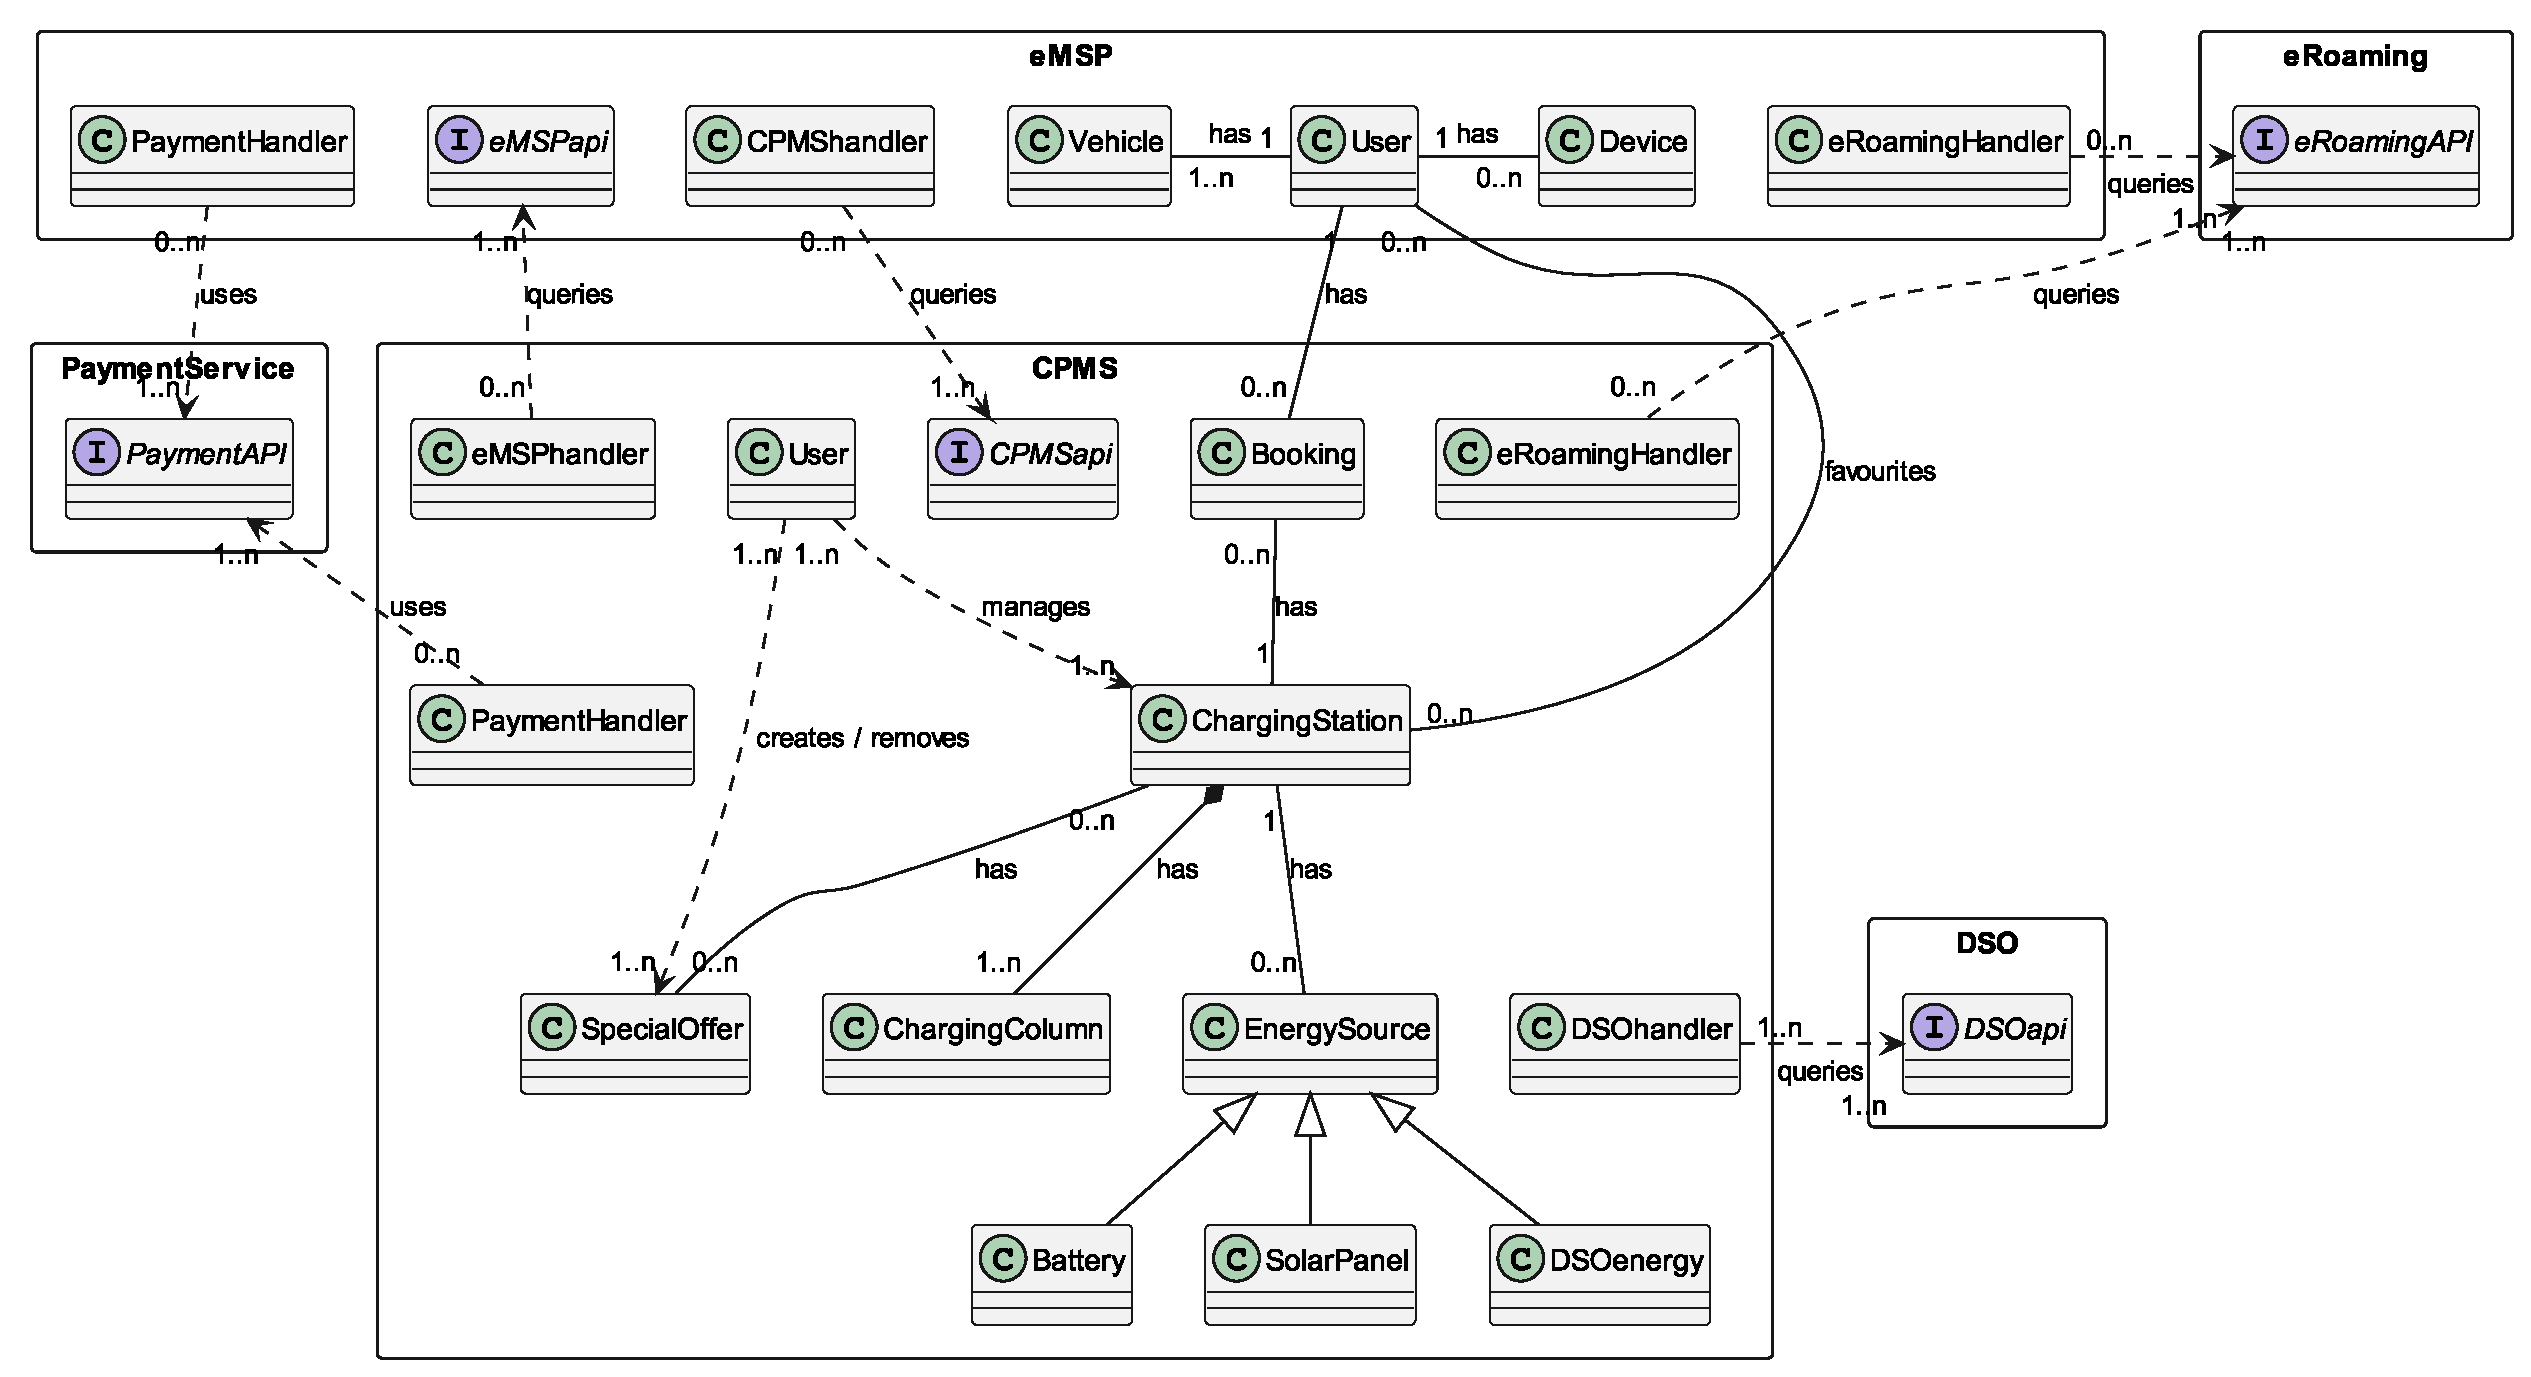
\includegraphics[width=0.99\columnwidth]{./images/diagrams/class}
    \caption{the class diagram of the various systems with the main interactions.}
\end{figure}

\pagebreak

\section{eMSP functions}

This section explains all the different functionalities that the eMSP provides to the end users (consumers).

\paragraph{Note} All the notifications that are mentioned in this section are in-app notifications (or emails, if the user selected this as the preferred notification method) that can be sent to the user only if there is at least one user's logged-in device with his/her credentials, otherwise, the email is chosen for the notification. If the notification derives from direct user interactions within the application, in-app notifications are sent only to the logged-in devices of the user which aren't the ones s/he has used to perform that action.

\subsection{Registration and login/logout}

Every new user who wants to register is asked to provide some basic information, like name, surname, birthdate, an email address that will be used as the username, and a password (which has to be given twice).\medskip

In case the email address is already present in the database or the two password fields don't coincide, the sign-up request is aborted, and the user is notified about this. If otherwise, the request ends successfully, the user receives an email at the specified address (username) with a confirmation link that expires within 24h from the emission. If the user doesn't confirm the address, the registration is automatically deleted. When the account is confirmed it becomes accessible through the login procedure and a confirmation email is sent to the user.\medskip

Every registered user can log into the system by providing username and password. If both are present in the database and the account has been confirmed, the user is granted access to his/her private area in which s/he can look for a charging station, book a charge or pay for it (and a few more other functionalities). Moreover, there is the possibility to log out. This deletes all the information stored locally on the user's device preventing him/her from accessing the account before logging in again.

\subsection{Look for nearby stations}

Every logged user can access a page with all the charging stations which can be sorted by distance (manually inserting the location or geolocalizing the user's device), by price (taking into account also any eventual discounts), or by availability. The user is also given the possibility to select a charging station, in which case the system will provide all the information related to that station, like the name, the precise location (address), the price for the charge, the number of parking slots for recharging and a calendar with all the availabilities (the available slots per period of time). Moreover, here is where the user is given the possibility to book a charge (which is described below in the next subsection).

\subsection{Book a charging station for a certain timeframe}

The booking of a charging slot is to be intended as the prosecution of the preceding subsection.\medskip

When the user wants to book a slot in a specific station, s/he selects the car s/he wants to charge (if more than one is associated), and the system gives him/her all the available consecutive time slots\footnote{Available consecutive time slots are adjacent time slots at a specific charging column. As an example, if there are only two available adjacent time slots related to two different charging columns at the same station, they aren't shown as a unique slot since the user would be forced to move the vehicle in the middle of the charge between the two columns.} for every day (with a fixed maximum look ahead from the current date). The system will try, as much as possible, to organize the physical slots according to the reservations, so it gives the user only an aggregated view of the availabilities. In any case, if the reservation ends successfully, the system sends a notification with the details of the reservation and the possibility to add it to the calendar.

\subsection{Receive important notifications}

15 minutes before the booked charge (or immediately if the user books a charge for that moment), the user receives a notification indicating the exact charging slot s/he has been assigned by the system for the charge.\medskip

Moreover, once the CPMS notices that the charging process of the user's vehicle is finished\footnote{This, of course, works only if the user booked that charging slot, otherwise, the system is structured in a way that it forbids the user to recharge the vehicle by simply not charging it.}, it informs the eMSP which sends a notification to the user, telling that the charge is finished, and that s/he can proceed in removing the socket and the vehicle from the charging zone and paying for the service.

\vfill

\subsection{Pay for the service}

After the charge is finished, the user is allowed to pay for the obtained service. This can be done through an apposite section in his/her personal area in the application or through a physical in-place device\footnote{The physical in-place device can be a POS (like pretty much on every vending machine at Politecnico di Milano) or another kind of device that allows payments.}. In any case, the user is notified once the payment is completed (both in case of success and failure). If the payment fails, the user can retry it, and this process repeats until the user successfully pays for the service.

\subsection{Query external services}

The system periodically queries an eRoaming service that informs it about all the available CPOs that subscribed to that network. From that moment on, the eMSP can interact with all their specific CPMSs, exchanging information thanks to the use of standard APIs.

\section{CPMS functions}

This section, instead, covers all the functionalities that the CPMS should provide to the authorized users of the CPO.

\subsection{Login/logout}

Every registered user can log into the system by providing a username and password. If a match is found in the database, the user is granted access to the area where s/he can manage the allowed charging station. Having logged in, the user can at any point log out from the website.

\subsection{Manage energy mix}

After login, users can define a new energy mix to be used by the system for a specific charge station. This includes defining from which sources energy is provided to sockets and if batteries are to be recharged, used, or ignored. Users can also let the system automatically define energy mixes that can change over time.

\subsection{Manage DSO choice}

After login, users can select what DSO is being used by the system, or let the system choose automatically based on the lowest rates. DSO rates can be queried from a list of available DSOs.

\subsection{Get info about a charging station's internal/external status}

After login, users can query information about a charging station's external status. This includes all available charging columns and relative sockets and how many cars are present. Users can also query information about a charging station's internal status. This includes amounts of energy available in its batteries, and for each charging vehicle, the amount of power absorbed and time left to the end of the charge.

\subsection{Manage special offers}

After login, users can create a new special offer by specifying a start date, an end date, and a discount amount. Special offers can be expanded in future versions of the system. Users can also delete an existing special offer, to make up for mistakes in the making of a new special offer.

\vfill
\pagebreak

\section{User characteristics} \label{users}

In this section are described all the various classes of users who are interacting with the system\footnote{For the sake of simplicity, the obvious superusers (the administrators) of each system are not presented here.}.

\subsection{Consumer (end user)}

The consumer is the end user of the eMSP system: s/he's the one that wants to charge an electric vehicle. The consumer can look for a charging station thanks to the use of a map integrated into the mobile application, and when s/he identifies a satisfying one (s/he can look for availability, price\dots), s/he can book a charge in a specific time slot at that station (if there is still any available). Once the charge is finished, s/he receives a notification from the application on the smartphone or, if preferred, an email. When s/he takes away the vehicle after the charge, s/he can pay for the obtained service, directly at the charging station or through an apposite function on the application.

\subsection{CPO's authorized user}

The CPO's authorized user is the end user of the CPMS system. S/he owns charging stations and can manage the charging columns via the CPMS. S/he can make decisions regarding which DSO to acquire energy from, change the cost of charges, set special offers, and decide how to direct the flow of energy in presence of multiple sources (for example if solar panels or batteries are available). S/he can also monitor the external and internal situation of charging stations, as to infer information about bottlenecks in the management of the system (for example if a station is always crowded it would be wise to consider expanding it with new charging columns) and information regarding the health of components (like in the case of local batteries).

\section{Domain assumptions}

These are all the domain assumptions done in order to write the specifications of this system.

\begin{center}
    \begin{tabular}{ | >{\centering\arraybackslash}m{0.1\columnwidth} | >{\arraybackslash}m{0.84\columnwidth} | }
        \hline
        \textbf{Identifier} & \multicolumn{1}{c|}{\textbf{Description}} \\
        \hline
        \hline
        \showD{d:connect} & Users can connect to the internet and access the service. \\
        \hline
        \showD{d:plug} & Consumers know how to manage the vehicle charging process, plugging and unplugging the vehicle. \\
        \hline
        \showD{d:remove} & Consumers remove their vehicles by the end of the booked charging slot. \\
        \hline
        \showD{d:truth} & Consumers provide true and correct information when registering on the platform. \\
        \hline
        \showD{d:vehicle} & Every vehicle that uses the system has a certificate used for authenticating it at the charging column and the consumer can access it. \\
        \hline
        \showD{d:dso} & DSOs provide true and correct data to CPOs. \\
        \hline
        \showD{d:abusive} & No one abusively parks in the slots. \\
        \hline
        \showD{d:harm} & No physical harm is done to the equipment at the charging stations. \\
        \hline
        \showD{d:unauthorized} & No unauthorized person can alter the state of the charging station (plugging and unplugging cables, opening the stations\dots). \\
        \hline
        \showD{d:batteries} & Batteries are durable/stable during the charging process (both in cars and charging stations). \\
        \hline
        \showD{d:dso_energy} & Charging stations are designed to not have energy shortages, even in case of full load. \\
        \hline
        \showD{d:socket} & All sockets types are compatible, but charge speed is not guaranteed for different types. \\
        \hline
        \showD{d:charge} & Sooner or later the charging process of every vehicle ends (the vehicle is fully charged, or the time slot is ended). \\
        \hline
        \showD{d:reliable} & There is a reliable network and structure to connect all the components outside the managed infrastructure. \\
        \hline
        \showD{d:payment} & All payments are handled by a third party and go through correctly (either commit or abort, notifying the result to both the user and the system). \\
        \hline
        \showD{d:api} & Uniform APIs already exist and are already implemented in the other systems in order to simplify the communication between all the different service providers. \\
        \hline
        \showD{d:cpo} & Only users authorized by CPOs can be given credentials to access the CPMS and manage it. \\
        \hline
        \showD{d:eroaming} & There exists an eRoaming service, already configured on the systems, that allows them to discover each other. \\
        \hline
    \end{tabular}
\end{center}
